\section{Referencial Teórico}
Nesta seção, serão apresentados os conceitos e ferramentas utilizados neste trabalho, através de uma revisão da literatura a fim assegurar a compreensão por completo do projeto. 

\subsection{CAPTCHA}

Desenvolvido em meados de 1997 para o site Alta Vista e, posteriormente para o Yahoo, o Captcha (Completely Automated Public Turing test to tell Computers and Humans Apart. Na tradução: Teste de Turing público completamente automatizado para diferenciação entre computadores e humanos) é utilizado como uma solução ferramenta de segurança anti-spam cuja premissa é utilizar uma mensagem distorcida como desafio para comprovar que o acessante é um ser humano, em vez de um robô / computador.

O Teste de Turing (postulado por  Alan Turing, em 1950) é uma forma de determinar se as atividades de máquina inteligentes podem ser assimiladas ao comportamento humano.  Qualquer sistema (incluindo o CAPTCHA)se converge em gerar questões nas quais apenas seres humanos e não os computadores, por mais inteligentes que sejam, não conseguiriam resolver. No caso do CAPTCHA, a pergunta desafio pode ser de referência à interpretação de mensagens alfanuméricas distorcidas em imagens, interpretação de objetos e cliques em partes específicas de uma imagem; partindo da premissa de que máquinas com inteligência artificial, por mais aperfeiçoadas que sejam, não conseguiriam interpretar de forma razoável.

\subsection{Aprendizado de Máquina}

Atualmente a produção de dados (imagens, textos, sons, vídeos, dentre outras fontes) está em crescimento. A maior distinção neste cenário é que as informações criadas / processadas ao redor do globo não são produzidas apenas por seres humanos, mas sim, dispositivos eletrônicos e aplicações. 

Devido a imensa quantidade de dados gerados, os seres humanos, incapacitados de interpretar tamanhas quantidades, terceirizam cada vez mais esta função para dispositivos dotados de inteligência artificial através do conceito de aprendizado de máquina que, por sua vez, utiliza-se de ferramentas e tecnologia que buscam responder perguntas e gerar insights através do consumo dados\cite{santos2018identificaccao}.

\subsubsection{Treinamento para Aprendizado de Máquina}

A premissa básica para todo aprendizado de máquina é o "treinamento" desta onde se usa dados previamente selecionados para criação e parametrização do determinado modelo de predição, que é usado para gerar previsões de resultados futuros de acordo com os estímulos que o agente inteligente receber \cite{russell2002artificial}. Contudo, para que o próprio treinamento seja satisfatório, os dados devem ser tratados previamente de modo a selecionar quais dados são importantes de fato para o aprendizado. Fato este que requer muito esforço \cite{russell2002artificial}.

\subsubsection{Aplicações do Aprendizado de Máquina}

A utilização de aprendizado de máquina é amplamente ut paira suas aplicilzações a fim de personalizar os seus produtos de forma automatizada para cada usuário, como em recomendação de vídeos, identificação fácil, sistemas de saúde, segurança, entre outras aplicações. Há três grandes categorias de aprendizado de máquina: supervisionado, não-supervisionado e reforço \cite{russell2002artificial}. Aqui, foi usado o aprendizado supervisionado, portanto esse será o foco.

\subsubsection{Aprendizado Supervisionado}

Neste tipo de aprendizado, os dados são rotulados, então eles são corretos para realizar o treinamento do modelo. Esse método é deveras eficiente, já que o sistema pode trabalhar com informações corretas \cite{russell2002artificial}. 

A rotulação dos dados é o cerne deste tipo de aprendizado, pois quando os rótulos são contínuos, então o problema é de regressão e quando forem discretos, então o problema é de classificação \cite{russell2002artificial}.

Vejamos dois exemplos:
\begin{enumerate}
    \item Regressão — Dada uma imagem de homem/mulher, tentar prever sua idade com base em dados da imagem.
    \item Classificação — Dada um exemplo de tumor cancerígeno, tentar prever se ele é benigno ou maligno através do seu tamanho e idade do paciente.
\end{enumerate}

Em resumo, o aprendizado supervisionado realiza um treinamento de um modelo por meio de um histórico de dados rotulados e realiza predições de outros dados futuros não rotulados \cite{santos2018identificaccao}, onde no primeiro exemplo seria a imagem de homem/mulher e no segundo exemplo as características de um tumor.

%\subsection{Redes Neurais Artificiais (RNA)}
\subsection{Redes Neurais Convolucionais (CNN)}
As Redes Neurais Convolucionais (\textit{Convolutional Neural Networks}, CNNs) foram propostas inicialmente em 1998, aonde os autores construíram uma arquitetura de rede neural chamada \textit{LeNet5}, utilizada para reconhecer dígitos escritos à mão \cite{lecun1998gradient}.

As CNNs são similares às redes neurais tradicionais, já que em ambos os casos são compostos por neurônios com seus respectivos pesos e bias que requerem treinamento \cite{haykin2007redes}. Cada neurônio é alimentado por algumas entradas. Em seguida é aplicado a ele o produto escalar das entradas e pesos, e uma função não-linear. 

O trunfo das CNNs está no tipo de entrada, imagens \cite{santos2018identificaccao}. Isso permite codificar propriedades na arquitetura da rede, distintivamente das redes neurais tradicionais, uma vez que esse último produz um número muito alto de pesos a serem treinados, tornando inviável e não escalável para o tipo de entrada imagem.

\subsubsection{Arquitetura}

A estrutura de uma CNN é composta por uma série de camadas. A primeira camada é a entrada (\textit{input}), usualmente sendo uma imagem com suas características de largura, altura e profundidade. Depois da entrada, vem três camadas próprias da CNN: camada convolucional, camada de \textit{pooling} e camada totalmente conectada. É também comum que exista a camada de ativação logo após a convolução  \cite{haykin2007redes}. A Figura \ref{fig:arch} demonstra a arquitetura de forma genérica.

\begin{figure}
    \centering
    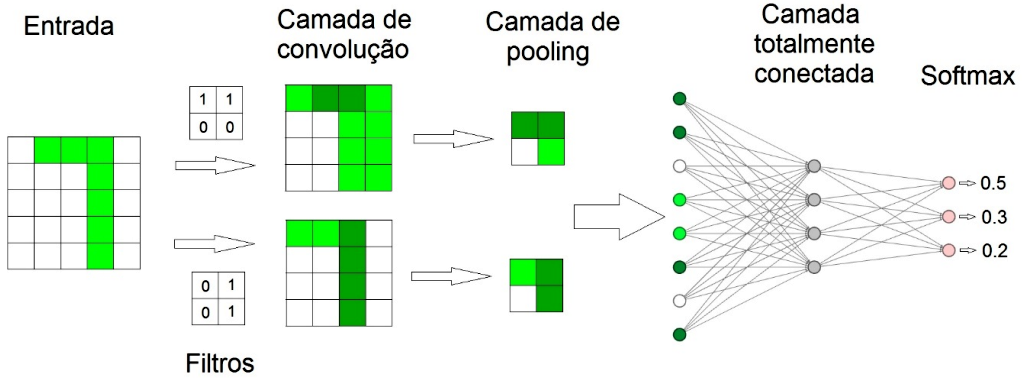
\includegraphics[scale=0.25]{Relatorio/figuras/arch.png}
    \caption{Arquitetura de uma CNN \cite{eliveltoebermamrenatoa.krohling2018}}
    \label{fig:arch}
\end{figure}

As CNNs são arquitetadas estritamente para reconhecimento de formas bidimensionais com um alto grau de invariância quanto a translação, escalonamento, inclinação e outras formas de distorção \cite{haykin2007redes}.

\subsubsection{Camada Convolucional}

A camada convolucional efetua a parcela mais pesada do processamento computacional. Nessa camada, cada neurônio não está ligado a todas as entradas da rede. Além disso, a camada é composta por um conjunto de filtros, que são pequenas matrizes de valores reais capazes de aprender de acordo com o treinamento. Por falar em treinamento dos filtros, nesse momento há operações de convolução para reconhecer a imagem de entrada e criar um mapeamento de características. Isso significa que, se o conjunto de valores de um filtro for capaz de retratar uma região da imagem, a rede como um todo compreende que estes mesmos valores poderão ser usados para identificar outra região da entrada se posto em outro filtro. Mesmo assim, os valores dos filtros variam ao longo do treinamento a fim de tecer reparos, adequações e executar melhores extrações de características de uma imagem de entrada.

\begin{figure}
    \centering
    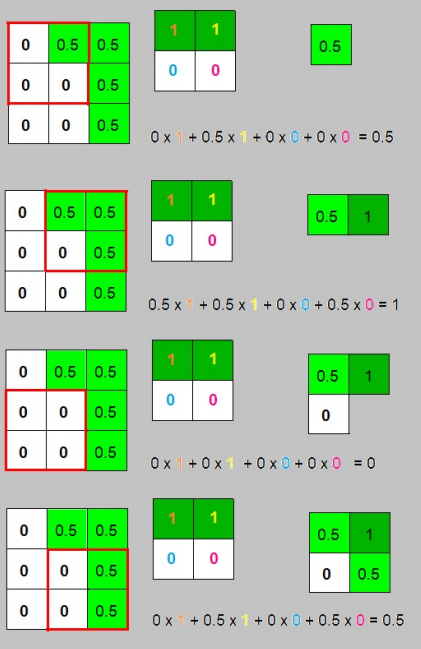
\includegraphics[scale=0.3]{Relatorio/figuras/stride.png}
    \caption{Operação de convolução e \textit{strides} em matrizes de entrada \cite{eliveltoebermamrenatoa.krohling2018}}
    \label{fig:stride}
\end{figure}

A Figura \ref{fig:stride} demonstra um fenômeno de deslizamento de quadro que seleciona uma quantidade de valores. Isso é orientado pelo parâmetro \textit{stride}. Na figura, o filtro desloca-se pela imagem 1 pixel por vez para os lados e para baixo. Às vezes o tamanho do filtro e do \textit{stride} não se adequam a imagem, tendo então que acionar o \textit{zero-padding}. Isso não é nada mais do que colocar zeros na borda da imagem para que o deslizamento ocorra \cite{haykin2007redes}.

A camada convolucional emprega muitos neurônios para esquematizar a entrada, mas em uma quantidade fixada. Por limitar a quantidade de neurônios, o número de conexões diminui, entretanto facilita a otimização dos parâmetros internos, os quais tornam-se mais importantes.

\subsubsection{Camada de \textit{Pooling}}

A camada de \textit{pooling}, em resumo, simplifica o resultado da camada antecessora. Da mesma forma que na convolução, é escolhida uma unidade de área para transitar por toda saída da camada anterior. Isso serve para resumir a informação de determinada área em um valor apenas (Figura \ref{fig:pooling}). Por exemplo, se a saída da camada anterior for 24x24 e a unidade de área definida for 2x2, então a saída do \textit{pooling} é uma matriz 12x12. Não basta apenas transitar, mas saber como será a sua sumarização. O meio mais empregado para isso é o \textit{maxpooling}, aonde apenas o maior número da unidade é enviado à saída. Isso serve para decrescer a quantidade de pesos a serem aprendidos e também evitar o \textit{overfitting}.

\begin{figure}
    \centering
    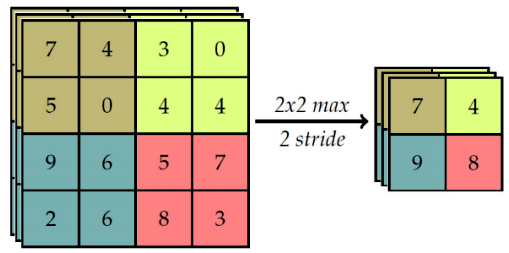
\includegraphics[scale=0.3]{Relatorio/figuras/pooling.png}
    \caption{\textit{Pooling} com \textit{maxpooling} \cite{santos2018identificaccao}}
    \label{fig:pooling}
\end{figure}


\subsubsection{Camada Totalmente Conectada}

Essa camada se caracteriza pela completude de conexões com a camada antecessora, onde sua entrada é a saída da camada anterior e sua saída são N neurônios, com N sendo a quantidade de classes do modelo para finalizar a classificação (Figura  \ref{fig:full}). É a última camada de uma CNN, já que atua do mesmo modo que as redes neurais tradicionais. É possível então adicionar as mesmas técnicas de melhoramento de desempenho da camada, como o \textit{dropout}, por exemplo \cite{eliveltoebermamrenatoa.krohling2018}.

\begin{figure}
    \centering
    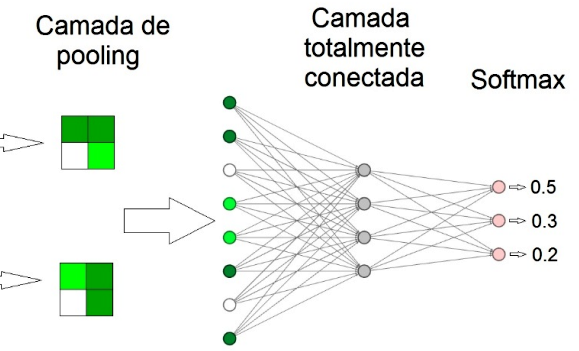
\includegraphics[scale=0.3]{Relatorio/figuras/full_conected.png}
    \caption{Camada totalmente conectada, com \textit{softmax} \cite{eliveltoebermamrenatoa.krohling2018}}
    \label{fig:full}
\end{figure}

Na saída (elemento mais ao extremo) é aplicada a função \textit{softmax} para se ter a probabilidade de dada entrada pertencer a uma certa classe (Figura \ref{fig:full}). Aqui é realizado o algoritmo de treinamento supervisionado \textit{backpropagation}. O erro obtido nesta camada é propagado para que os pesos dos filtros das camadas convolucionais sejam ajustados. Assim, os valores dos pesos compartilhados são aprendidos ao longo do treinamento.


\subsection{Funções de Ativação}

Funções de ativação basicamente decidem se um neurônio deve ser ativado, ou não. É a transformação não-linear que é feita ao longo do sinal de entrada. Esta saída é então encaminhada como entrada para a próxima camada de neurônios. A função de ativação faz a transformação não-linear dos dados de entrada, sendo possível então a rede aprender a executar tarefas mais complexas (Processamento de linguagem natural, Visão computacional etc) \cite{haykin2007redes}. 

\subsubsection{Função Unidade Linear Retificada (ReLU)}
\subsubsection{Função SoftMax}

\subsection{Função de otimização Adam}
\subsection{Overfitting}
\subsection{Dropout}
\subsection{Matriz de Confusão}

\subsection{Ferramentas}
\subsubsection{Tensorflow}
\subsubsection{Keras}

\subsubsection{Numpy}

O NumPy é uma poderosa biblioteca Python que é usada principalmente para realizar cálculos em Arrays Multidimensionais. O NumPy fornece um grande conjunto de funções e operações de biblioteca que ajudam os programadores a executar facilmente cálculos numéricos. Esses tipos de cálculos numéricos são amplamente utilizados em tarefas como:

Modelos de Machine Learning: Ao escrever algoritmos de Machine Learning, supõe-se que se realize vários cálculos numéricos em Array. Por exemplo, multiplicação de Arrays, transposição, adição, etc. O NumPy fornece uma excelente biblioteca para cálculos fáceis (em termos de escrita de código) e rápidos (em termos de velocidade). Os Arrays NumPy são usados para armazenar os dados de treinamento, bem como os parâmetros dos modelos de Machine Learning.

Processamento de Imagem e Computação Gráfica: Imagens no computador são representadas como Arrays Multidimensionais de números. NumPy torna-se a escolha mais natural para o mesmo. O NumPy, na verdade, fornece algumas excelentes funções de biblioteca para rápida manipulação de imagens. Alguns exemplos são o espelhamento de uma imagem, a rotação de uma imagem por um determinado ângulo etc.

Tarefas matemáticas: NumPy é bastante útil para executar várias tarefas matemáticas como integração numérica, diferenciação, interpolação, extrapolação e muitas outras. O NumPy possui também funções incorporadas para álgebra linear e geração de números aleatórios. É uma biblioteca que pode ser usada em conjuto do SciPy e Mat-plotlib. Substituindo o MATLAB quando se trata de tarefas matemáticas.

\subsubsection{OpenCV}

OpenCV (Open Source Computer Vision) é uma biblioteca de programação, de código aberto e inicialmente desenvolvida pela Intel com o objetivo de tornar a visão computacional mais acessível a desenvolvedores e hobistas. Atualmente possui mais de 500 funções, pode ser utilizada em diversas linguagens de programação (C++, Python, Ruby, Java…) e é usada para diversos tipos de análise em imagens e vídeos, como  detecção, tracking e reconhecimento facial, edição de fotos e vídeos, detecção e análise de textos, etc. 

\subsubsection{Matplotlib}